%%%%%%%%%%%%%%%%%%%%%%%%%%%%%%%%%%%%%%%%%%%%%%%%%%%
%
%  Author: Jacob Vaughn
%  
%  Last Updated: 3/8/2024
%
%%%%%%%%%%%%%%%%%%%%%%%%%%%%%%%%%%%%%%%%%%%%%%%%%%%

%%%%%%%%%%%%%%%%%%%%%%%%%%%%%%%%%%%%%%%%%%%%%%%%%%%%%%%%%%%%%%%%%%%%%%
%%               EXPERIMENTAL APPROACH & OBJECTIVES
%%%%%%%%%%%%%%%%%%%%%%%%%%%%%%%%%%%%%%%%%%%%%%%%%%%%%%%%%%%%%%%%%%%%%

\chapter{EXPERIMENTAL APPROACH \& OBJECTIVES}

\section{Experimental Control and Efficiency Improvements} 

Stuff about ACE2.0 controls

\subsection{Feedback-Controlled Mach Number Selection}

Inputting Mach number into PLC to actively adjust to desired Mach number within some tolerance. Result of above ACE2.0 development.


Unsure how to proceed; review \cite{stephens-hubbard}.

\subsection{Reynolds Number Control Scheme}

Control $P_{0}$ to maintain constant Re/m during Mach sweep. Look into anticapatory change in Re/m for potential delayed response time in $P_{0}$, and look into potential proportional Re/m change to model acceleration or altitude change.

Mathematic model predictive controller or preprogrammed controller will be implemented until an adequate PID controller can be developed.

\begin{equation}
    Re/m = \frac{\rho U}{\mu}
\end{equation}
\begin{equation}
    \frac{T_0}{T} = (1+\frac{\gamma-1}{2}M^2) = F
\end{equation}
\begin{equation}
    \frac{P_0}{P} = (1+\frac{\gamma-1}{2}M^2)^{\frac{\gamma}{\gamma+1}} = F^{\frac{\gamma}{\gamma+1}}
\end{equation}
\begin{equation}
    \rho = \frac{P}{R T} = \frac{P_0 F^{\frac{-\gamma}{\gamma-1}}}{R T_0 F^{-1}} = \frac{P_0}{R T_0 F^{\frac{1}{\gamma-1}}}
\end{equation}
\begin{equation}
    U = M \sqrt{\gamma R T} = M F^{-\frac{1}{2}} \sqrt{\gamma R T_0}
\end{equation}
\begin{equation*}
    Re/m = \frac{\rho U}{\mu} = \frac{1}{\mu} \frac{P_0}{R T_0 F^{\frac{1}{\gamma-1}}} M F^{-\frac{1}{2}} \sqrt{\gamma R T_0}
\end{equation*}
\begin{equation}
    Re/m = \sqrt{\frac{\gamma}{R T_0}} \frac{M P_0}{\mu} F^{-\frac{\gamma+1}{2(\gamma -1}}
\end{equation}

For constant Re/m assuming $\gamma, R, T_0 = const.$ and with $\frac{dF}{dt} = (\gamma-1)M \frac{dM}{dt}$:
\begin{equation}
    \frac{d(Re/m)}{dt} = 0 = P_0 \frac{dM}{dt} + M \frac{dP_0}{dt} - \frac{M P_0}{\mu} \frac{d\mu}{dt} - \frac{\gamma+1}{2} M^2 P_0 F^{-1} \frac{dM}{dt}
\end{equation}

Sutherland's Law with $T_\mu = 273$, $S_\mu = 111$, and $\mu_0 = 1.716 \times 10^{-5}$:
\begin{equation}
    \mu = \mu_0 \frac{T_\mu+S_\mu}{T+S_\mu} \left( \frac{T}{T_\mu} \right)
\end{equation}
\begin{equation}
    \mu = \frac{\mu_0(t_\mu+S_\mu)}{T_\mu^{\frac{3}{2}}} \frac{T_0^{\frac{3}{2}} F^{-\frac{3}{2}}}{T_0 F^{-1}+S_\mu}
\end{equation}
\begin{equation}
    \frac{\frac{d\mu}{dt}}{\mu} = (\gamma-1) M F^{-1} \frac{dM}{dt} \left( \frac{T_0 F^{-1}}{T_0 F^{-1} + S_\mu}-\frac{3}{2} \right)
\end{equation}

Substiuting and solving for $\frac{dP_0}{dt}$:
\begin{equation}
    \frac{dP_0}{dt} = P_0 M F^{-1} \frac{dM}{dt} \left[ (\gamma-1) \left( \frac{T_0 F^{-1}}{T_0 F^{-1} + S_\mu} - \frac{3}{2} \right) + \frac{\gamma+1}{2} - \frac{1}{M^2 F^{-1}} \right]
\end{equation}

While this model is ..., the actual controls may not be physically implented by the author due to time constraints and the fact that the M6QT shares the air supply controls. Installing controllable valve would disrupt testing in both facilities.

\section{Nozzle Noise and Uniformity Characterization with Hysteresis}

In order to establish a baseline for future work within the ACE2.0 facility, a pitot survey was performed to measure and characterize the freestream noise and uniformity throuhgout the nozzle. Utilize pitot probe/rake and kulites mounted on traverse to characterize entire nozzle exit plane and centerline into nozzle up to 24??? inches upstream of nozzle exit.

Sweep Re/m and Mach to explore hysteresis of noise and maybe uniformity. Begin with Re/m sweep up and back down in current ACE.

The characterization test matrix is shown in Table \ref{tab:ace2-survey}. These runs are divided into a few distinct objectives: (1) uniformity, (2) uncerntainty, (3) pressure fluctiation transition, and (4) hysteresis. The last seven runs will be replicates of the first seven to quantify the uncerntainty in pressure fluctuations, Mach number, and uniformity.

\begin{figure}[ht]
    \centering
    \begin{subfigure}[b]{0.4\textwidth}
            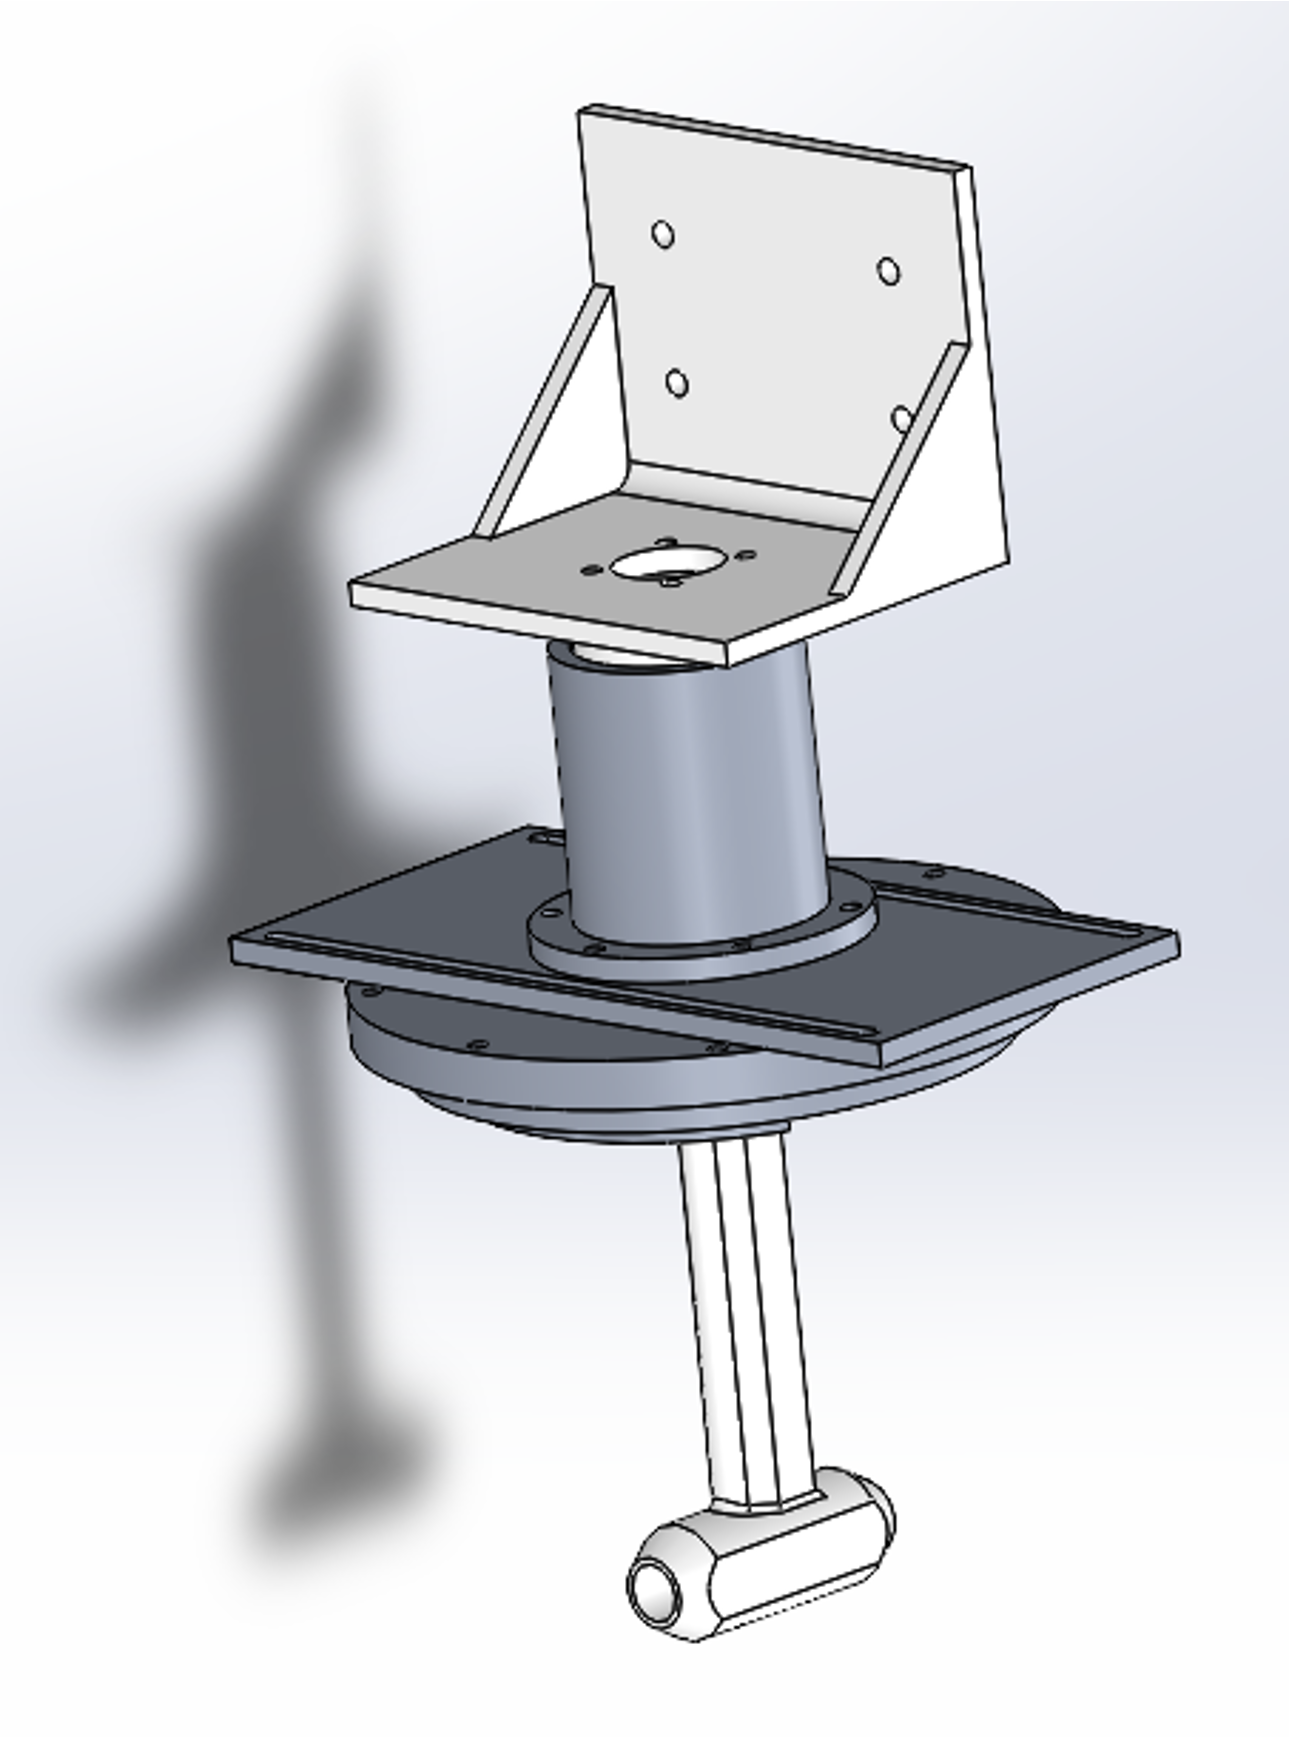
\includegraphics[width=\textwidth]{traverse-x}
        \caption{X traverse}
        \label{fig:traverse-x}
    \end{subfigure}
    \begin{subfigure}[b]{0.22\textwidth}
            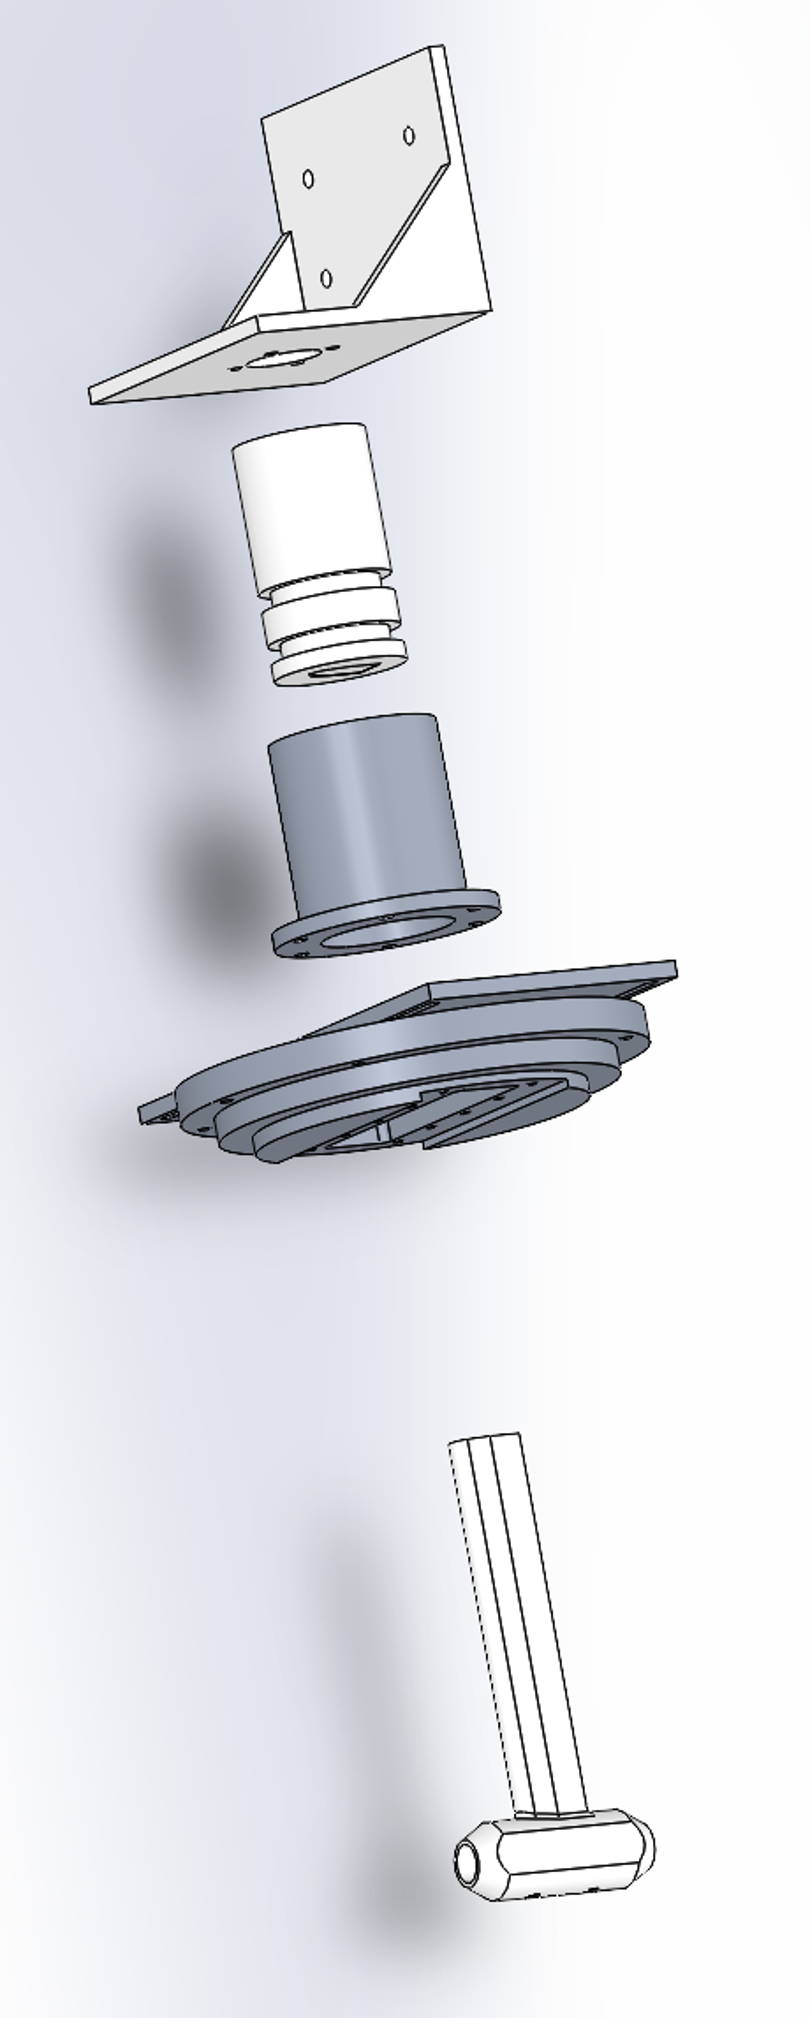
\includegraphics[width=\textwidth]{traverse-explode}
        \caption{Exploded assembly}
        \label{fig:traverse-explode}
    \end{subfigure}
    \begin{subfigure}[b]{0.35\textwidth}
            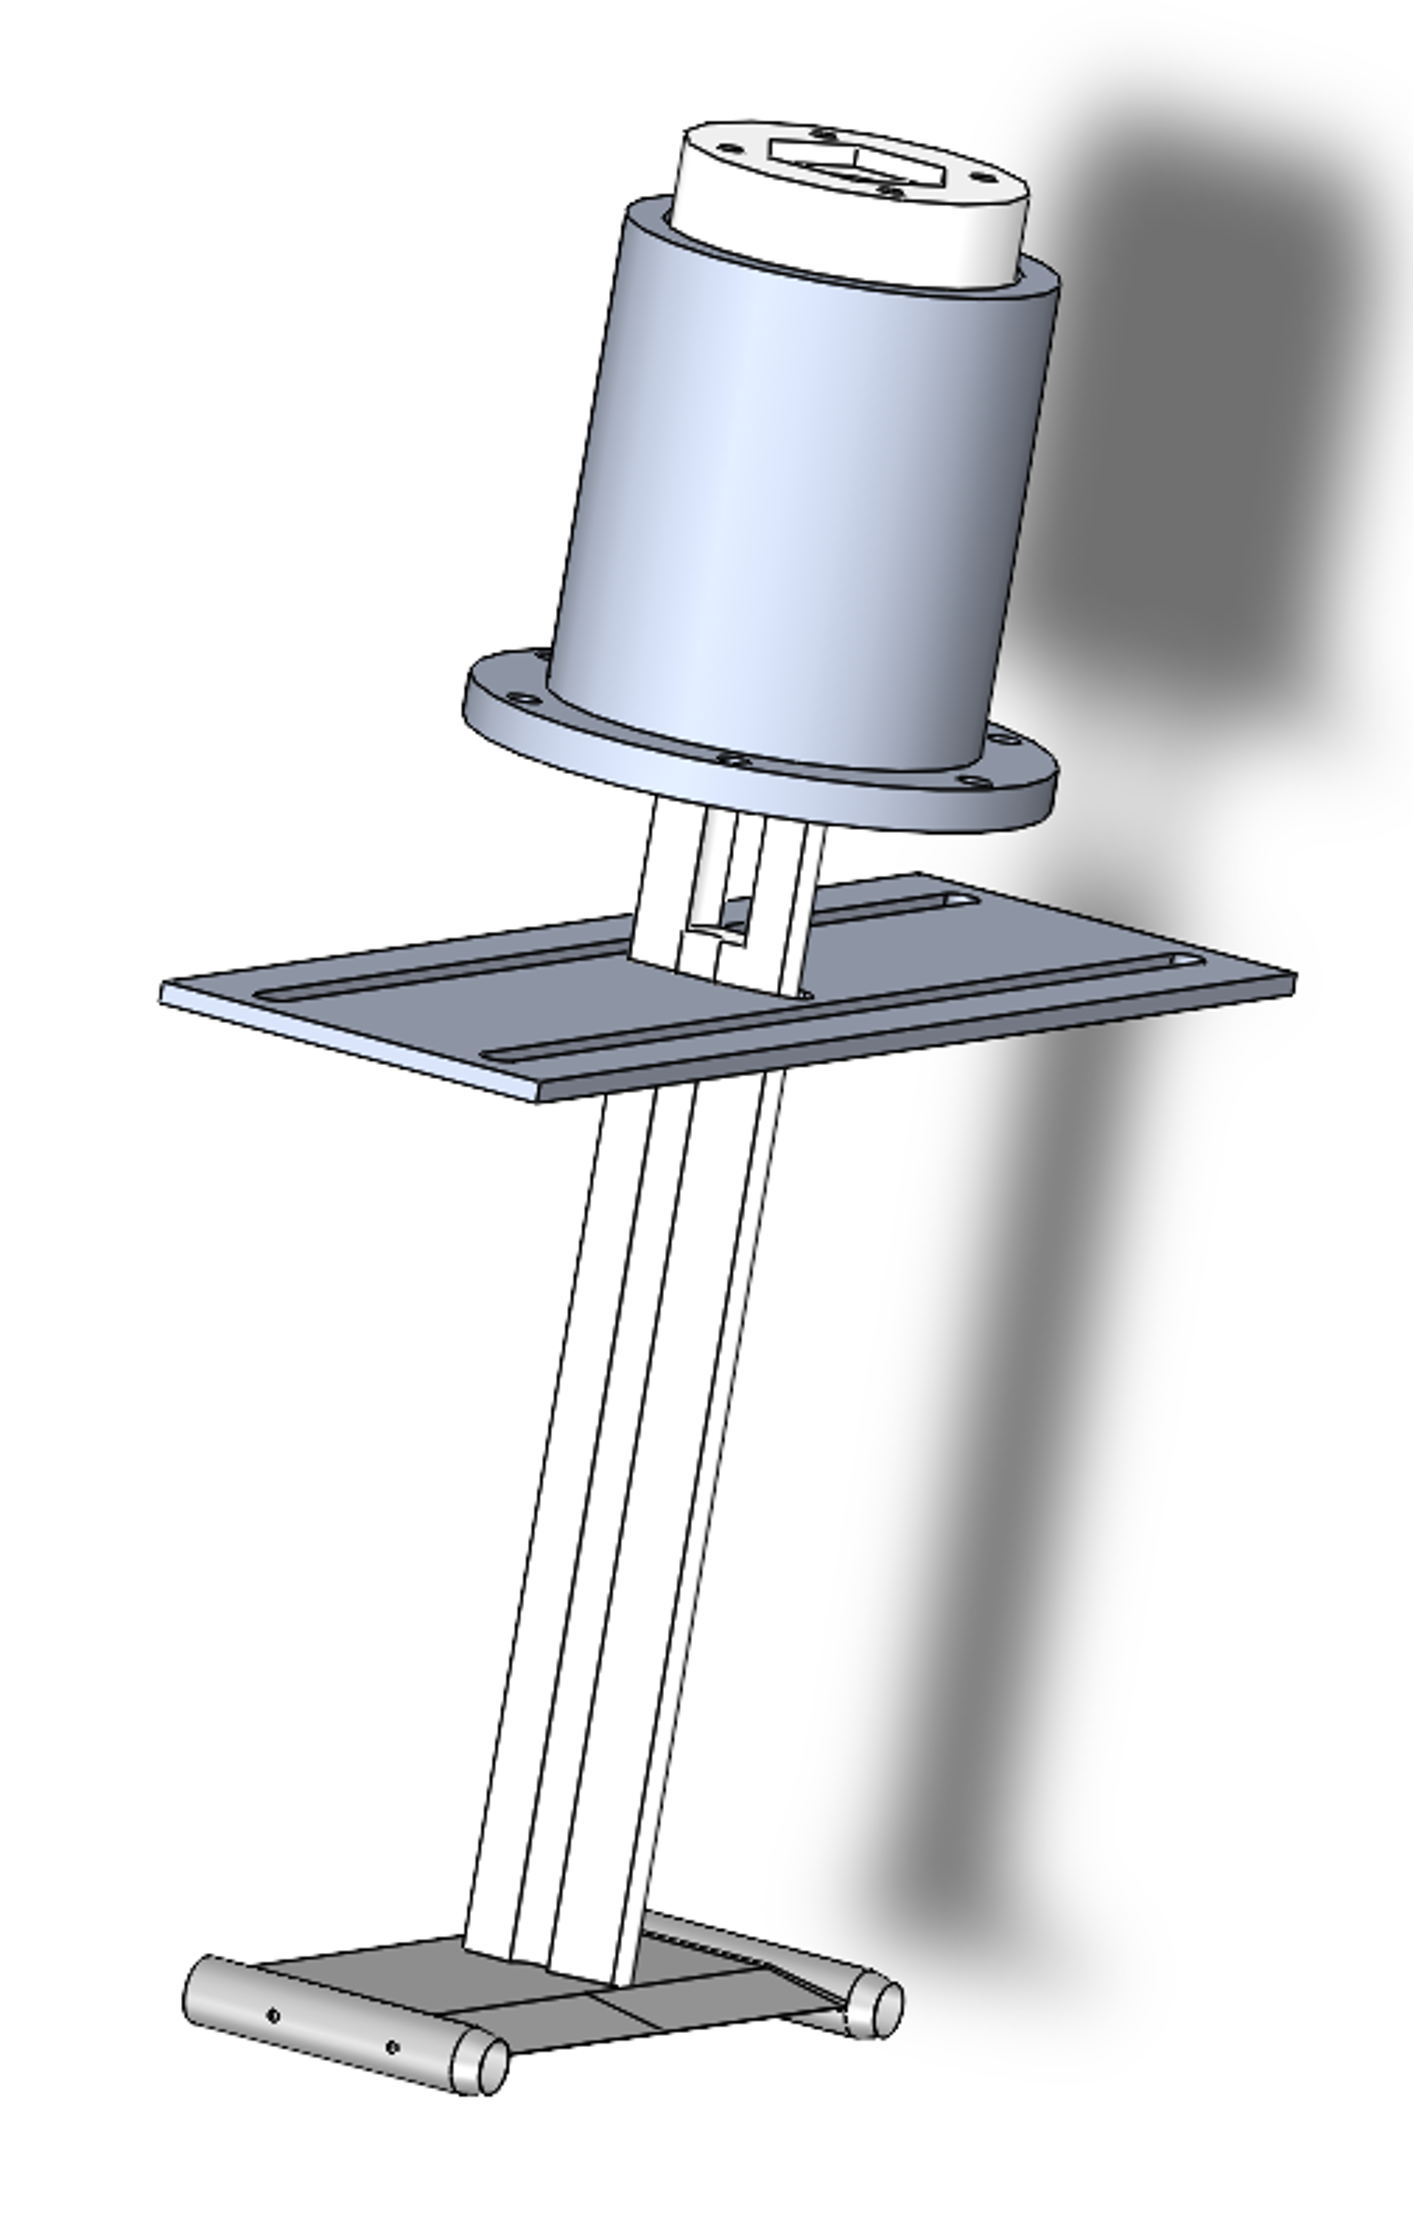
\includegraphics[width=\textwidth]{traverse-y}
        \caption{Y-traverse}
        \label{fig:traverse-y}
    \end{subfigure}
    \caption{Traverse configurations}
    \label{fig:traverse}
\end{figure}

\begin{figure}[ht]
    \centering
    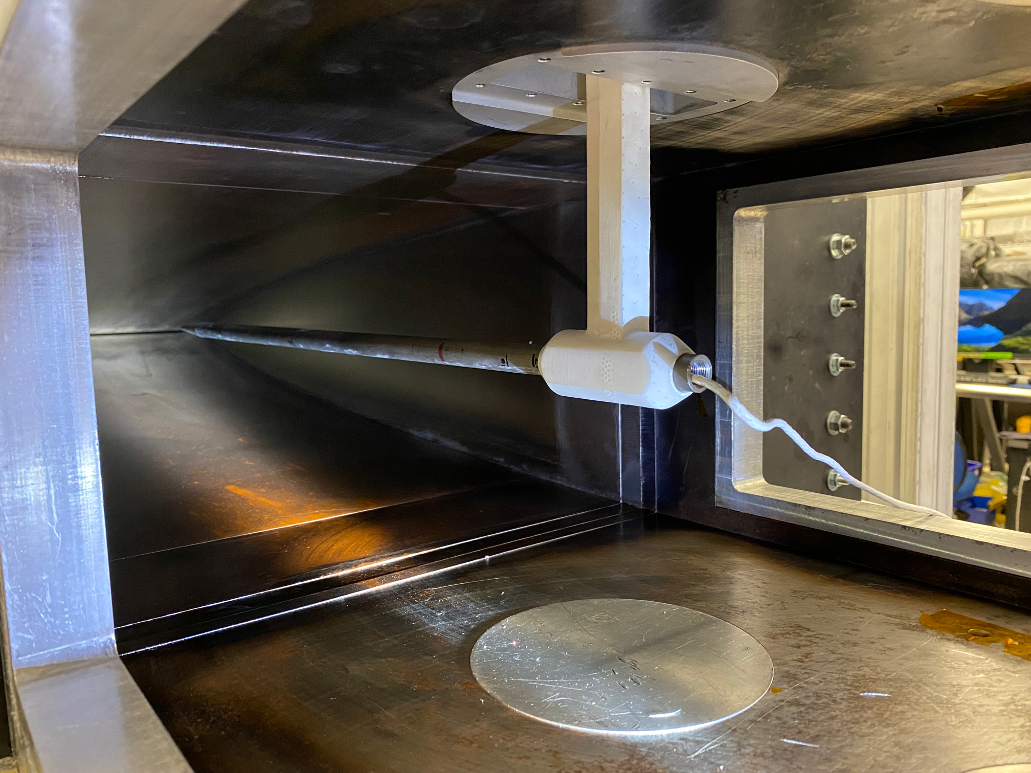
\includegraphics[width=6in]{pitot17}
    \caption{Pitot probe measuring 17 in. upstream of nozzle exit.}
    \label{fig:pitot17}
\end{figure}

\begin{table}[ht]
    \centering
    \label{tab:ace-survey}
    \begin{tabular}{|c|c|c|c|c|}
        \hline
    \textbf{Run} & \textbf{X (in.)} & \textbf{Y (in.)} & \textbf{Z (in.)} & \textbf{Re/m ($\times10^6$)} \\ \hline
        1 & 0 & 0 & 0 & 2$\to$7$\to$2 \\ \hline
        2 & -17 & 0 & 0 & 2$\to$7$\to$2 \\ \hline
        3 & -24 & 0 & 0 & 2$\to$7$\to$2 \\ \hline
    \end{tabular}
    \caption{Test matrix for preliminary noise hysteresis in ACE.}
\end{table}

\begin{table}[ht]
    \centering
    \label{tab:ace2-survey}
    \begin{tabular}{|c|c|c|c|c|c|}
        \hline
        \textbf{Run} & \textbf{X (in.)} & \textbf{Y (in.)} & \textbf{Z (in.)} & \textbf{Mach} & \textbf{Re/m ($\times10^6$)} \\ \hline
        1 & 0 & 0 & 0 & 6 & 2$\to$7$\to$2 \\ \hline
        2 & 0 & 0 & 0 & 5$\to$8$\to$5 & 3 \\ \hline
        3 & 0 & -3 & -3:1:3 & 6 & 3 \\ \hline
        4 & 0 & -1.5 & -3:1:3 & 6 & 3 \\ \hline
        5 & 0 & 0 & -3:1:3 & 6 & 3 \\ \hline
        6 & 0 & 1.5 & -3:1:3 & 6 & 3 \\ \hline
        7 & 0 & 3 & -3:1:3 & 6 & 3 \\ \hline
        8 & -6 & 0 & 0 & 6 & 2$\to$7$\to$2 \\ \hline
        9 & -6 & 0 & 0 & 5$\to$8$\to$5 & 3 \\ \hline
        10 & -6 & -3 & -3:1:3 & 6 & 3 \\ \hline
        11 & -6 & -1.5 & -3:1:3 & 6 & 3 \\ \hline
        12 & -6 & 0 & -3:1:3 & 6 & 3 \\ \hline
        13 & -6 & 1.5 & -3:1:3 & 6 & 3 \\ \hline
        14 & -6 & 3 & -3:1:3 & 6 & 3 \\ \hline
        15 & -17 & 0 & 0 & 6 & 2$\to$7$\to$2 \\ \hline
        16 & -17 & 0 & 0 & 5$\to$8$\to$5 & 3 \\ \hline
        17 & -24 & 0 & 0 & 6 & 2$\to$7$\to$2 \\ \hline
        18 & -24 & 0 & 0 & 5$\to$8$\to$5 & 3 \\ \hline
        19 (1) & 0 & 0 & 0 & 6 & 2$\to$7$\to$2 \\ \hline
        20 (2)& 0 & 0 & 0 & 5$\to$8$\to$5 & 3 \\ \hline
        21 (3) & 0 & -3 & -3:1:3 & 6 & 3 \\ \hline
        22 (4) & 0 & -1.5 & -3:1:3 & 6 & 3 \\ \hline
        23 (5) & 0 & 0 & -3:1:3 & 6 & 3 \\ \hline
        24 (6) & 0 & 1.5 & -3:1:3 & 6 & 3 \\ \hline
        25 (7) & 0 & 3 & -3:1:3 & 6 & 3 \\ \hline
    \end{tabular}
    \caption{Test matrix for ACE2.0 characterization and noise hysteresis study.}
\end{table}

\subsection{Uncerntainty Quantification}

Reference \cite{stephens-hubbard}

\subsection{Hysteresis}

Stuff

\section{Model Flow Characteristics Hysteresis During Mach Trajectory and Oscillation}

This objective serves as a demonstration of capabilities for ACE2.0. 

Look into hysteresis of boundary layers, shock interactions, and subsequent surface heat flux. 

Use fin-cone model for public and HARV for army and verbal?

\begin{figure}[ht]
    \centering
    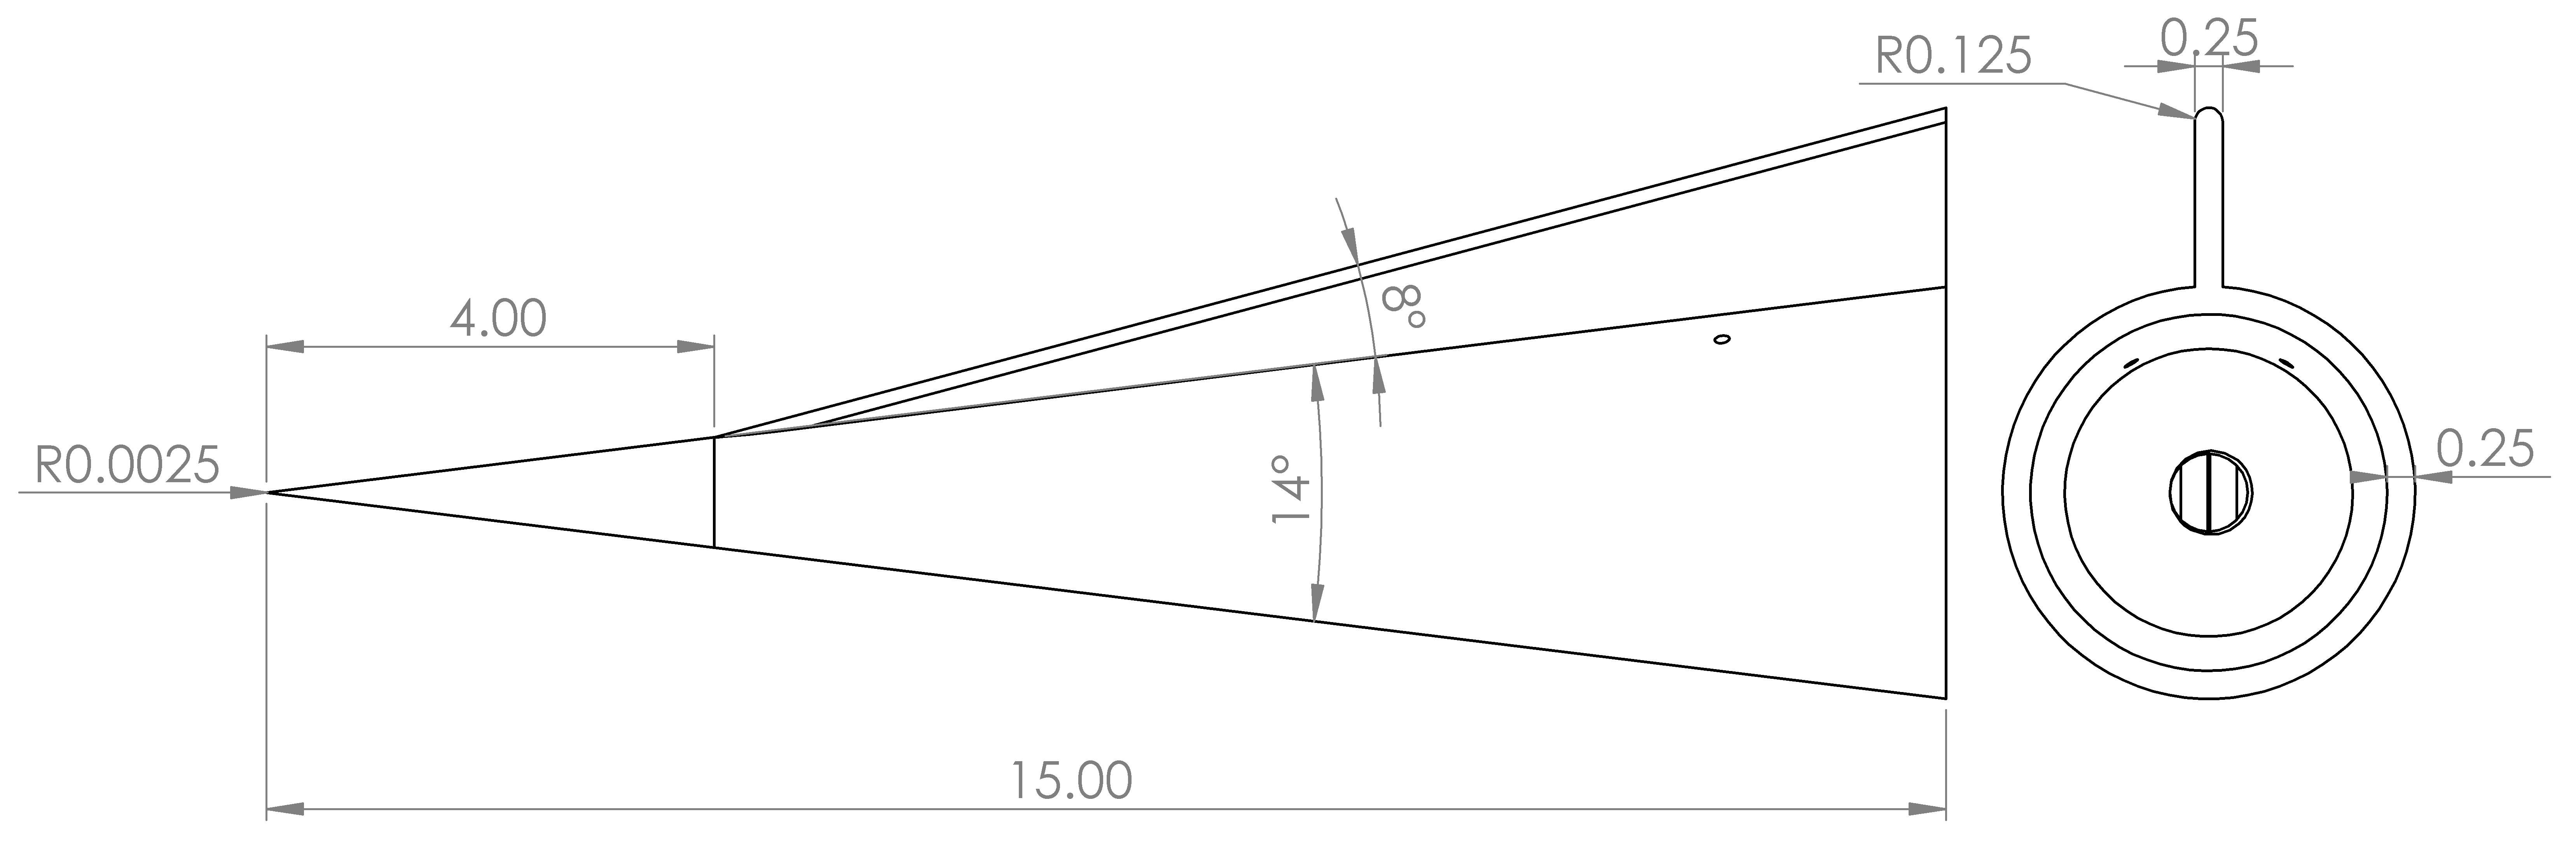
\includegraphics[width=6.5in]{fin-cone}
    \caption{Drawing of 7$\degree$ half-angle fin-cone model used for heat flux hysteresis study.}
    \label{fig:fin-cone}
\end{figure}

